\chapter{Revisão Bibliográfica}

No presente capítulo, são apresentados conceitos básico para a compreensão do presente trabalho. Nessa etapa, busca-se através da revisão de trabalhos já elucidados a contextualização do projeto proposto.

\section{Conceitos Básicos}

%Esta seção desenvolverá conceitos fundamentais para a compreensão da problemática resolvida com o sistema proposto. O objeto de estudo emerge à evidência quando observados dois atores opostos: a complexidade do sistema e sua robustez. Estes são primeiramente compreendidos pela natureza de um sistema embarcado.

Esta seção explanará conceitos bás

%%%%%%%%%%%%%%%%%%%%%%%%%%%%%%%%%%%%%%%%%%%%%%%%%%%%%%%%%%%%%%%%%%%%%%
\section{Sistemas de Controle}

%conceitos de resposta em frequência
% estabilidade de sistemas
% em regime
% diferentes tipos de sistemas

%%%%%%%%%%%%%%%%%%%%%%%%%%%%%%%%%%%
\subsection{Resposta ao Degrau}

\begin{figure}[htb]
  \caption{Representação do Modelo de Controlador PID com distúrbios}
  \begin{center}
      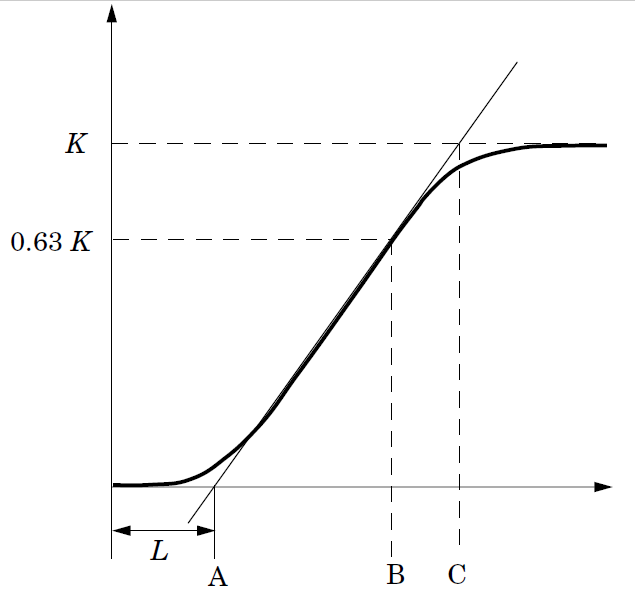
\includegraphics[scale=0.5]{img/transient_astrom_p17}
  \end{center}
  \fonte{Adaptado de \citeonline{Astrom1995}.} 
\end{figure}

\begin{figure}[htb]
  \caption{Representação do Modelo de Controlador PID com distúrbios}
  \begin{center}
      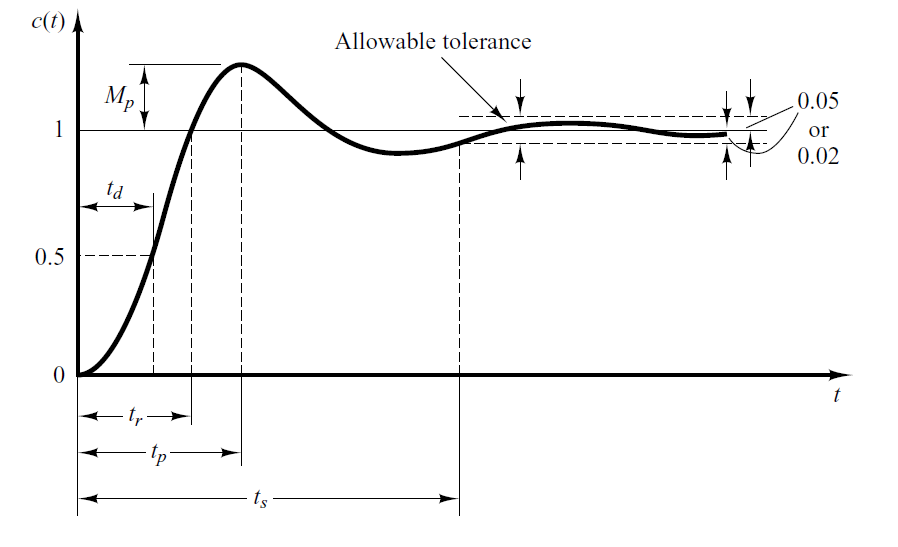
\includegraphics[scale=0.5]{img/transient_ogata_p170}
  \end{center}
  \fonte{Adaptado de \citeonline{Ogata}.} 
\end{figure}

%%%%%%%%%%%%%%%%%%%%%%%%%%%%%%%%%%%%%%%%%%%%%%%%%%%%%%%%%%%%%%%%%%%%%%
\section{Controladores}

\begin{figure}[htb]
  \caption{Representação do Modelo de Controlador PID com distúrbios}
  \begin{center}
      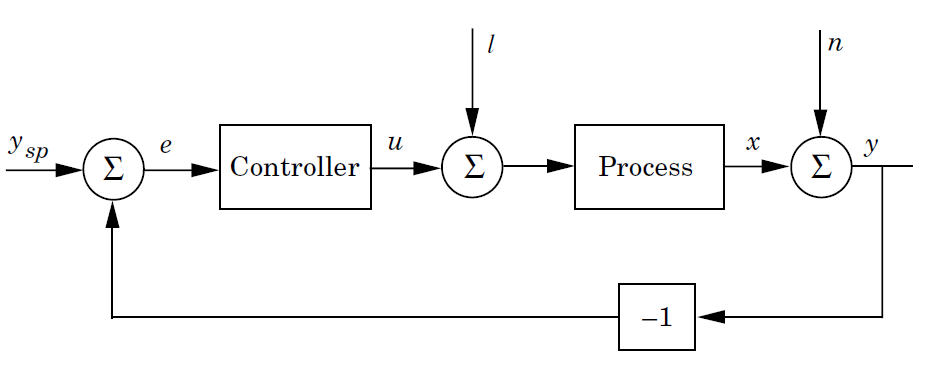
\includegraphics[scale=0.65]{img/feedback_loop_astrom_p65}
  \end{center}
  \fonte{Adaptado de \citeonline{Astrom1995}.} 
\end{figure}

\begin{figure}[htb]
  \caption{Representação do Modelo de Controlador PID com distúrbios}
  \begin{center}
      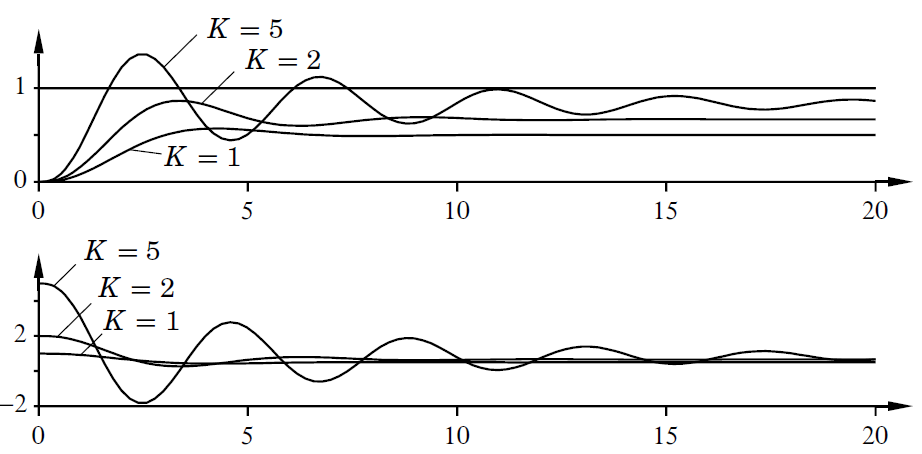
\includegraphics[scale=0.65]{img/proportional_astrom_p66}
  \end{center}
  \fonte{Adaptado de \citeonline{Astrom1995}.} 
\end{figure}

%%%%%%%%%%%%%%%%%%%%%%%%%%%%%%%%%%%%%%%%%%%%%%%%%%%%%%%%%%%%%%%%%%%%%%
\subsection{Sintonia de Controladores}


%%%%%%%%%%%%%%%%%%%%%%%%%%%%%%%%%%%%%%%%%%%%%%%%%%%%%%%%%%%%%%%%%%%%%%
\subsection{Controladores PID}

\begin{figure}[htb]
  \caption{Representação do Modelo de Controlador PID com distúrbios}
  \begin{center}
      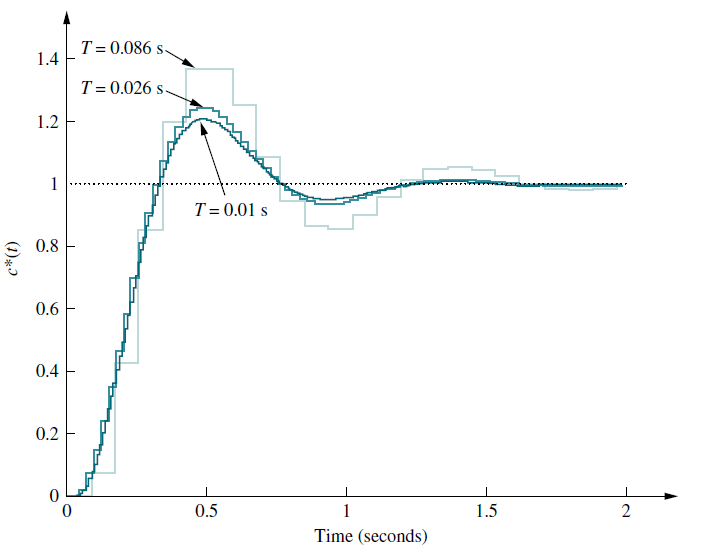
\includegraphics[scale=0.65]{img/nise_digitalinput_p761}
  \end{center}
  \fonte{Adaptado de \citeonline{Nise}.} 
\end{figure}

\begin{figure}[htb]
  \caption{Representação do Modelo de Controlador PID com distúrbios}
  \begin{center}
      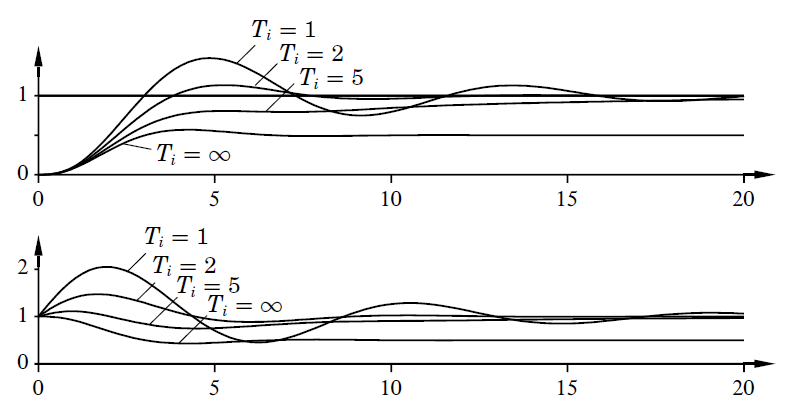
\includegraphics[scale=0.75]{img/pi_astrom_p68}
  \end{center}
  \fonte{Adaptado de \citeonline{Astrom1995}.} 
\end{figure}

\begin{figure}[htb]
  \caption{Representação do Modelo de Controlador PID com distúrbios}
  \begin{center}
      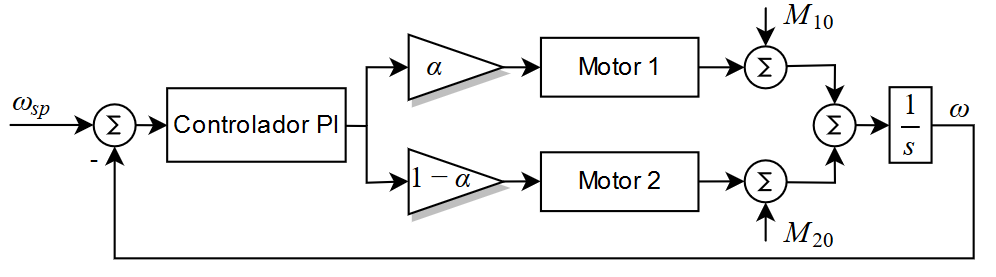
\includegraphics[scale=0.65]{img/pi_twomotors_astrom_p308}
  \end{center}
  \fonte{Adaptado de \citeonline{Astrom1995}.} 
\end{figure}

\begin{figure}[htb]
  \caption{Representação do Modelo de Controlador PID com distúrbios}
  \begin{center}
      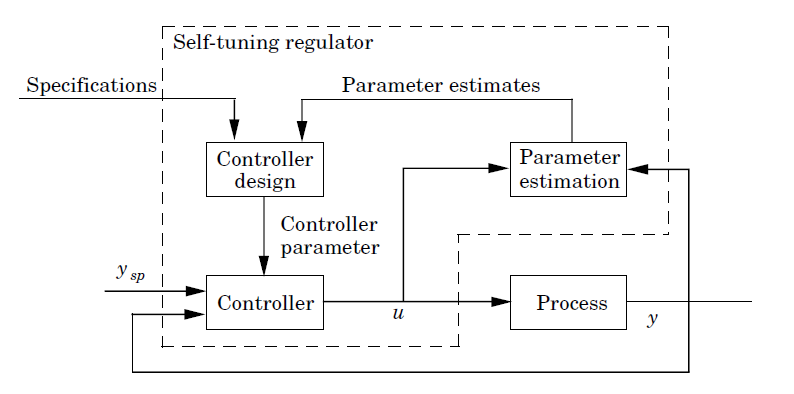
\includegraphics[scale=0.75]{img/pid_adaptative_astrom_p233}
  \end{center}
  \fonte{Adaptado de \citeonline{Astrom1995}.} 
\end{figure}

\begin{figure}[htb]
  \caption{Representação do Modelo de Controlador PID com distúrbios}
  \begin{center}
      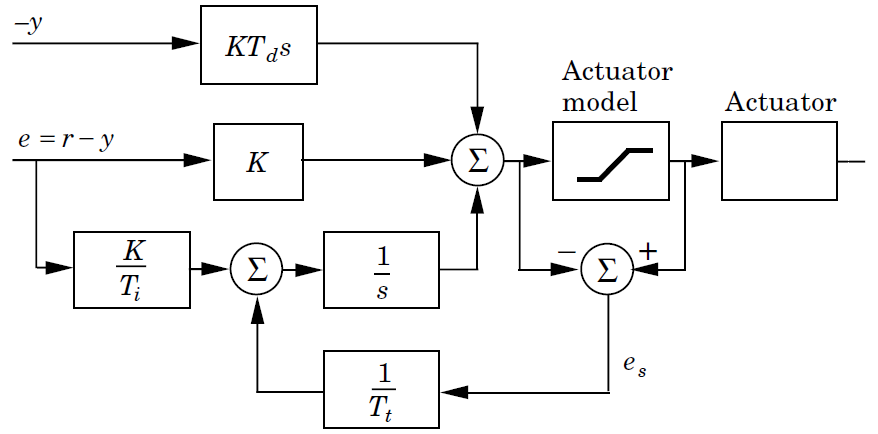
\includegraphics[scale=0.65]{img/pid_antiwindup_astrom_p83}
  \end{center}
  \fonte{Adaptado de \citeonline{Astrom1995}.} 
\end{figure}

\begin{figure}[htb]
  \caption{Representação do Modelo de Controlador PID com distúrbios}
  \begin{center}
      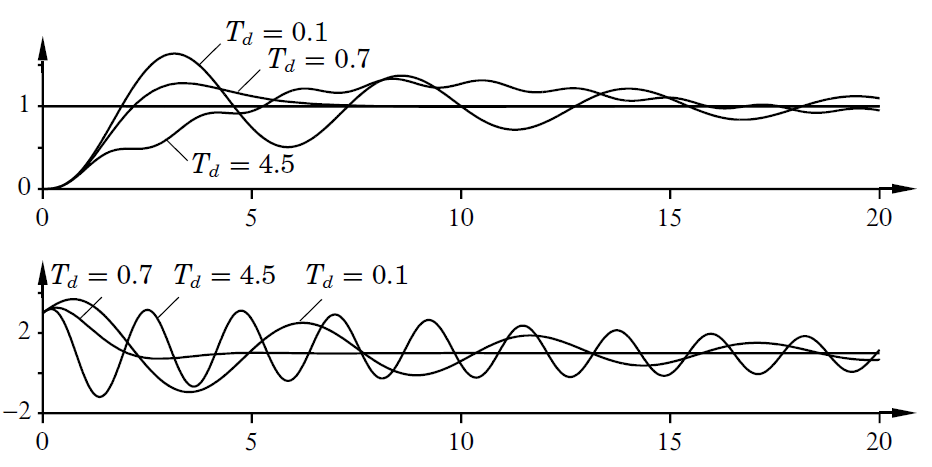
\includegraphics[scale=0.65]{img/pid_astrom_p70}
  \end{center}
  \fonte{Adaptado de \citeonline{Astrom1995}.} 
\end{figure}

\begin{figure}[htb]
  \caption{Representação do Modelo de Controlador PID com distúrbios}
  \begin{center}
      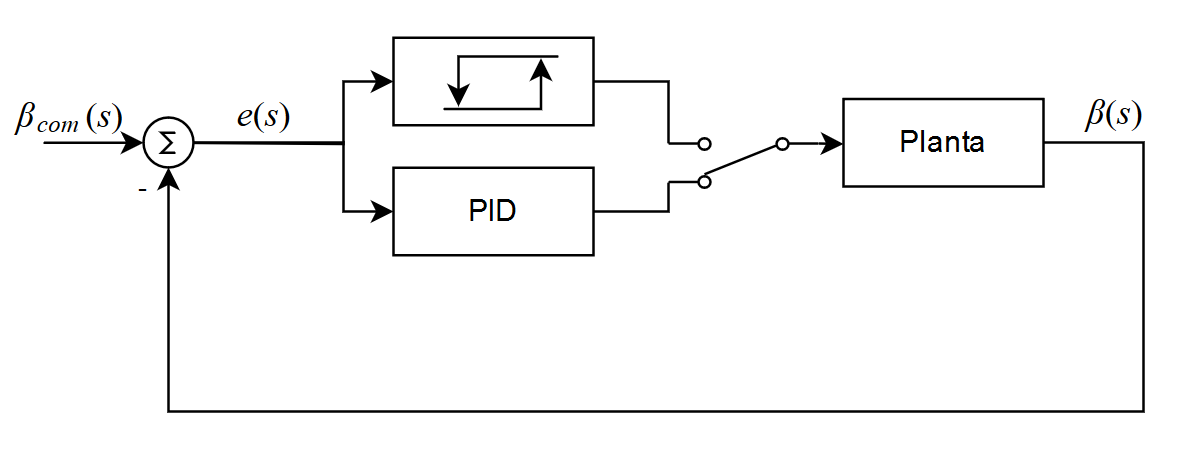
\includegraphics[scale=0.75]{img/pid_autotuning_relay_astrom_p239}
  \end{center}
  \fonte{Adaptado de \citeonline{Astrom1995}.} 
\end{figure}

\begin{figure}[htb]
  \caption{Representação do Modelo de Controlador PID com distúrbios}
  \begin{center}
      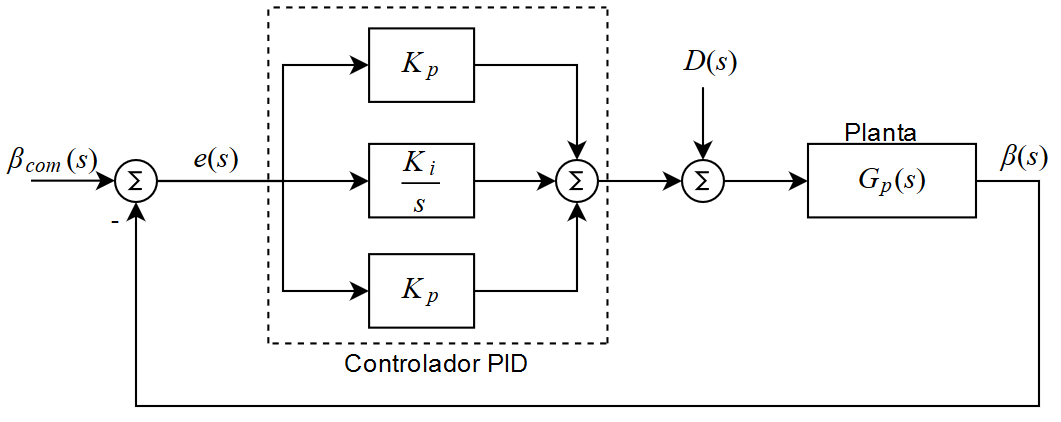
\includegraphics[scale=0.75]{img/pid_controller_Snider_p35}
  \end{center}
  \fonte{Adaptado de \citeonline{Snider}.} 
\end{figure}

%%%%%%%%%%%%%%%%%%%%%%%%%%%%%%%%%%%
\subsection{Método de sintonia de Ziegler-Nichols}

%%%%%%%%%%%%%%%%%%%%%%%%%%%%%%%%%%%
\subsection{Outras configurações de controladores PID}

%%%%%%%%%%%%%%%%%%%%%%%%%%%%%%%%%%%%%%%%%%%%%%%%%%%%%%%%%%%%%%%%%%%%%%
\section{Controle Inteligente}

%%%%%%%%%%%%%%%%%%%%%%%%%%%%%%%%%%%
\subsection{Lógica Fuzzy}

%%%%%%%%%%%%%%%%%%%%%%%%%%%%%%%%%%%
\subsection{Controle com Redes Neurais}  %control hand p1017

%%%%%%%%%%%%%%%%%%%%%%%%%%%%%%%%%%%%%%%%%%%%%%%%%%%%%%%%%%%%%%%%%%%%%%
\section{Satélites}

%%%%%%%%%%%%%%%%%%%%%%%%%%%%%%%%%%%
\subsection{Dinâmica rotacional de um Satélite}

\begin{figure}[htb]
  \caption{Representação do Modelo de Controlador PID com distúrbios}
  \begin{center}
      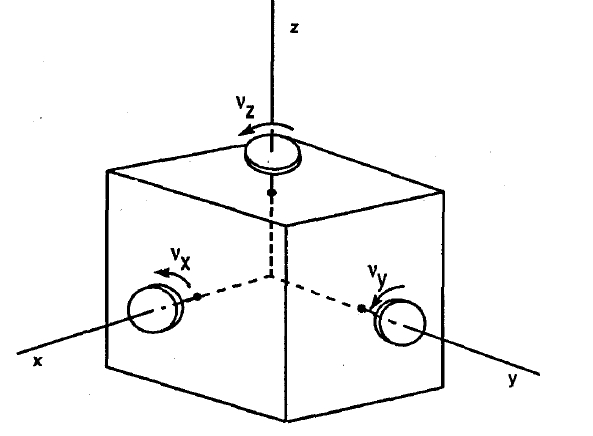
\includegraphics[scale=0.75]{img/satellite_controlhand_p1306}
  \end{center}
  \fonte{Adaptado de \citeonline{Levine1996}.} 
\end{figure}

%%%%%%%%%%%%%%%%%%%%%%%%%%%%%%%%%%%%%%%%%%%%%%%%%%%%%%%%%%%%%%%%%%%%%%
\section{Sistemas Embarcados}

%%%%%%%%%%%%%%%%%%%%%%%%%%%%%%%%%%%
\subsection{Comportamento Assíncrono}

%%%%%%%%%%%%%%%%%%%%%%%%%%%%%%%%%%%
\subsection{Threds}

%%%%%%%%%%%%%%%%%%%%%%%%%%%%%%%%%%%%%%%%%%%%%%%%%%%%%%%%%%%%%%%%%%%%%%
\section{Estado da Arte}

%%%%%%%%%%%%%%%%%%%%%%%%%%%%%%%%%%%
\subsection{Sistemas Inteligentes de Sintonia de Controladores}

\begin{figure}[htb]
  \caption{Representação do Modelo de Controlador PID com distúrbios}
  \begin{center}
      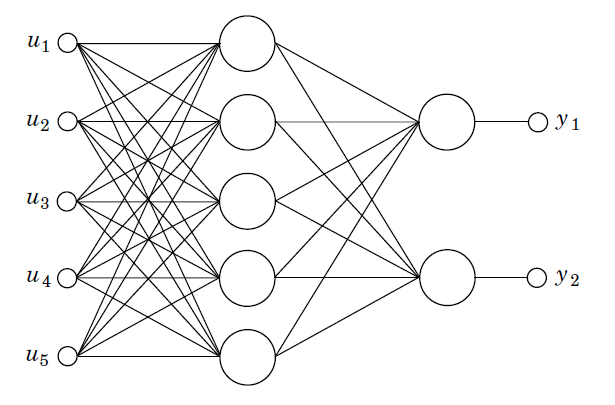
\includegraphics[scale=0.65]{img/feedforward_neural_astrom_p297}
  \end{center}
  \fonte{Adaptado de \citeonline{Astrom1995}.} 
\end{figure}

\begin{figure}[htb]
  \caption{Representação do Modelo de Controlador PID com distúrbios}
  \begin{center}
      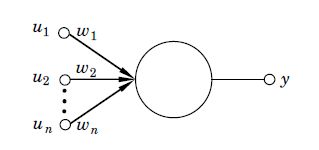
\includegraphics[scale=0.6]{img/neuron_astrom_p295}
  \end{center}
  \fonte{Adaptado de \citeonline{Astrom1995}.} 
\end{figure}

\begin{figure}[htb]
  \caption{Representação do Modelo de Controlador PID com distúrbios}
  \begin{center}
      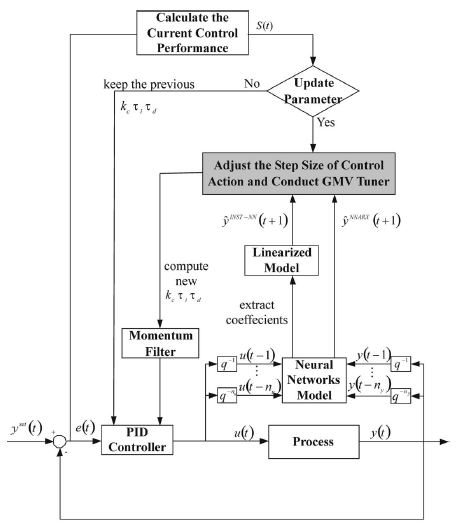
\includegraphics[scale=1]{img/pid_neural_Applying_p18}
  \end{center}
  \fonte{Adaptado de \citeonline{Chen2004}.} 
\end{figure}

%%%%%%%%%%%%%%%%%%%%%%%%%%%%%%%%%%%%%%%%%%%%%%%%%%%%%%%%%%%

